%\addcontentsline{toc}{chapter}{Development Process}
\chapter{Methods}
\section{Introduction}
This chapter is concerned with introducing the concepts and methodologies we will be using to complete this project. The aim is to familiarise the viewer with the theory behind our experiments, as well as hopefully to illustrate, in clear and concise terms, the motivation and methods behind them. This, combined with the next chapter, will give a complete overview of the experiment design and implementation which form the core of this project.

\section{The Importance of Data in Machine Learning}
For any ML problem the first and most important problem after determining the problem itself is deciding on the data.

Any ML algorithm begins with data $\left(Training Data\right)$ and ends with data $\left(Test Data, Performance Data\right)$. The purpose of machine learning is to extract information based on examples, so without examples it would be impossible to progress.

Of course that's not all we use data for. In order to evaluate our models, data is also used to drive other aspects of the ML lifecycle. We also need data to evaluate our model's performance, and our performance data is itself a very important data decision in ML.

When it comes to data having more of it is usually best, but there are cases where less, better quality data is more important. Indeed, unless data is of sufficient quality we cannot use it. Quality in this sense refers to our ability to learn from it. There are many qualities a set of data might possess that might make its quality poor.

If for example we train a model to classify between dogs and cats but have only 1 example of a cat for every 10 dogs, then perhaps our model will perform poorly, while in other tasks that's not really an issues. Different qualities of data are needed or desirable for different tasks.

Performance data is important as it  allows us to validate decisions and to direct our efforts in such a way as to achieve good general performance which is usually the objective in ML, the use of a trained model to map new examples to a learned output.

A data driven approach to problems is essential in ML.
\section{Dataset}
A dataset is a set of data that is to be used as inputs for an ML algorithm either for Training, Testing, or both. A dataset will usually consist of a set of inputs and a set of outputs.

What those sets of inputs and outputs are will depend on the type of dataset and potentially the problem  the dataset is designed to solve. For instance a dataset might be a set of images of Donald Trump and pictures of assorted barnyard animals, labeled as 'trump' and 'not-trump' This dataset might be suitable to train a model to identify pictures of Donald Trump.

If we wished to use a dataset like this to identify individual animals we might struggle however. In simple terms an ML algorithm can only learn things contained in the dataset it trains on. This creates a demand for many datasets to be created for many different purposes.

Creating, Normalising, and Evaluating a Dataset is a hard and complicated task, involving a lot of labour. Yet datasets are numerous as the problems they wish to solve. Choosing the correct dataset then goes hand in hand with selecting a problem.

\section{Artificial Neural Networks}
\subsection{Introduction}
Artificial Neural Networks are a series of ML models and methods that are based on a naive model of the biological function of neurons. They have origins as early as the 1940s \cite{citeulike:1295398} when Mathematical Biophysicists were studying the functions of neurons and were attempting to model them mathematically.

Neural Networks have progressed tremendously since those days but many of the fundamental concepts remain the same. At their core they still have basic simulated neurons and they still are trying to completely emulate the functions of a real neuron whether than be human, cat, or another organism.

As the name implies an ANN is a Network of Artificial Neurons, the way these neurons are connected to each other and 'fire' give them their properties including abilities to 'learn'. The way ANN's learn is quite useful for many problems where ML is traditionally applied.

Especially advantageous is an ANN's ability to learn without the need for feature extraction. Indeed ANNs are well known for being able to recognise patterns in even raw data.

The main disadvantage touted on the other hand is that because everything happens inside the ANN it is very hard to understand what your model is actually doing. This has lead to several anecdotes like Google's ANN learning that birds have branches as part of their legs, or some researchers that were trying to detect tanks from photos which ended up teaching their ANN that desert sceneries mean tank.

Of course this is not completely true and it the last few years we have seen a lot of research being done on this exact same topic. The days of ANNs being blackboxes is almost over.

While ANN is an umbrella term for this type of model there are many components that serve different functions or try to emulate different features of biological brain. Some of these components and models will be detailed in the following sections.

\subsection{Optimisers}
An optimisation function is one of the core concepts of ML. Its purpose is quite simple. To optimise the weights such that the ML algorithm learns. For our Networks we will be looking at one of many options that are available. Stochastic Gradient Descent.

Stochastic Gradient descent works by computing the negative gradient of the cost function by tracing through the network and then back-propagating through the true label. The main benefit of SGD over normal gradient descent is that it updates one value at a time which makes it really efficient especially to train on batches which reduce the computation overhead significantly.\cite{lecun1998gradient}

The second benefit is they are suitable for online learning which we will not be looking at in this report.
\subsection{Loss Functions}
\subsection{Activation Functions}
Activation functions are the parts of the ANN that give its neurons their biological like property. Real Neurons do not just fire when stimulated. Instead they have complicated chemical thresholds and other mechanisms that determine whether a neuron fires passing a message along to another in the network.

Activation Functions together with weighs are meant to simulate this mechanism. We will explain two of the ones we will be using bellow.

\subsubsection{ReLU}
\subsubsection{Softmax}

\subsection{Perceptrons}
A perceptron, or fully connected perceptron is one of the most basic ANN architectures available. It consists of an input layer of neurons, one or more 'hidden layers', and finally an output layer.

\begin{wrapfigure}{r}{0.32\textwidth}
	\begin{center}
		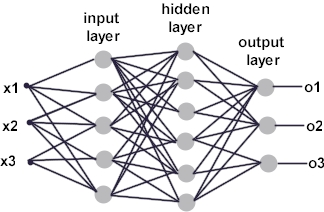
\includegraphics[width=0.30\textwidth]{ann}
	\end{center}
	\caption{Single Layer Perceptron}
    \hyperlink{http://dms.irb.hr/tutorial/tut_nnets_short.php}{Source}
	\label{mlp}
\end{wrapfigure}

We call it a fully connected model because each layer is connected to every neuron of every adjacent layer. This structure is reflected in figure \ref{mlp} Perceptron Networks with more than 1 layer are called Multi-Layer Perceptrons, or MLP for short.

Multi-Layer Perceptrons are quite powerful networks on their own and until a few decades ago were the dominant ANN in use, for many tasks they still perform quite well, while they have a few key disadvantages in vision problems like the problem we are addressing.

An MLP requires as many input neurons as there are channels so for an RGB image of size 32x32 we would need 3072 inputs because each of those inputs is fully connected that means that the number of calculations that is necessary can grow quite quickly.

For simple solving tasks this is not really an issue and as we will discuss later MLPs are still used as a component in a CNN.

\subsection{Convolutional Neural Networks}
A Convolutional Neural Network, otherwise referred to as a CNN is a type of Neural Network that has been available since around the 1990s. It is inspired by studies on how the cat visual system works.\cite{lecun1998gradient} It is quite common in ML literature and especially in the world of ANNs to find references to Biology.

A common ANN structure works by collecting coarse features through a series of Convolutional Filters which are aggregated via pooling. Then this is fed back to a set of finer filtering which extract more features. The process is repeated until the desired detail is extracted and the outputs are fed through an MLP and converted to answers for our ANN.

A cat's visual cortex works much the same by extracting features with increased detail as it goes from input to output.

Feature Maps and Convolutions work on two concepts. Sparse connectivity and encouraging locality. Neurons are made such that they only connect with neurons that are near in their 'visual field' this is justified because more often than not 'interesting things' tend to be quite near each other, an object will usually be a single body and so on so forth.

The main genefit of a CNNs approach is it can extract more information from an image than an MLP alone can while being relative inexpensive to build. Despite of this benefit, practical ANNs have only been around for a few years with Computer Scientists like LeCan trying to promote their use in computer vision \cite{lecun2010convolutional}. The advent of GPU compute has also been revolutionary in the field.

Because of their involvement one of the basic CNN designs has come to be know as LeNet.
\subsubsection{Structuring a CNN}

\begin{wrapfigure}{l}{0.50\textwidth}
	\begin{center}
		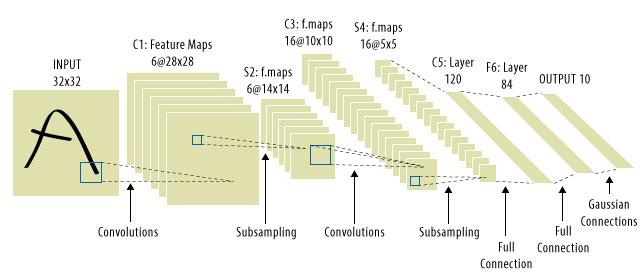
\includegraphics[width=0.48\textwidth]{common_cnn_design}
	\end{center}
	\caption{Example of a common CNN design.} \hyperlink{http://systemdesign.altera.com/can-you-see-using-convolutional-neural-networks/}{Source}
	\label{CNNModel}
\end{wrapfigure}

As we previously discussed a CNN consists of a number of layers figure \ref{CNNModel} illustrates the model. We have 2 or more feature layer, followed by a pooling layer, usually max pooling, followed by more feature layers. The feature layers are just convolutions.

Max pooling layers work by taking n inputs and outputting their max value. So suppose you had a max pooling layer of a pooling of 2x2, what would happen is you get 1 output with the max activation of 4 neurons.

With each iteration of this you accumulate features such that at the end your MLP can solve the feature maps to associate them to outputs. Depending on the type of problem the solutions are put into a different kind of output layers. In a multi-label classification problem like outs we woudl use something such as softmax from which the probabilities are mapped to classes.

\section{Network training}
One of the ways of training a neural network is through the Stochastic Gradient Descent Optimizer. What we will be focusing on  with this report is two concepts, an epoch, a period of time where out ANN encounters the complete set of training data and gets evaluated with optimisations applied, and a batch.

For each epoch, we go through each batch which is a portion of the total training images and optimise our neural network weights. The Neural Network trains by completing each epoch successfully until it is time to stop. Hyper Parameters like the bach-size, momentum, and learning rate affect this significantly but we decided to keep these locked after some early tweaking and focus on different optimisations.

\section{Network evaluation}
\subsection{Confusion Matrices}
\begin{wrapfigure}{r}{0.50\textwidth}
	\begin{center}
		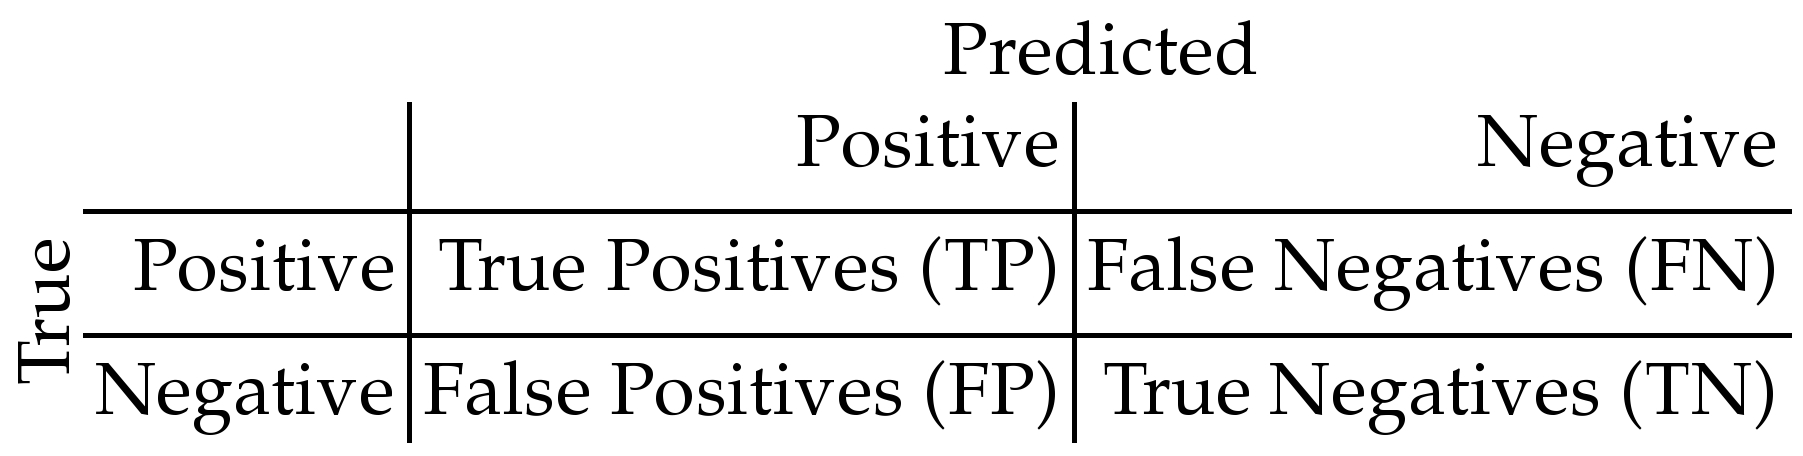
\includegraphics[width=0.48\textwidth]{confusion_example}
	\end{center}
	\caption{Example of a confusiong matrix}
	\hyperlink{http://www.intechopen.com/books/advances-in-data-mining-knowledge-discovery-and-applications/selecting-representative-data-sets}{Source}
	\label{cme}
\end{wrapfigure}
A confusion matrix is a way of representing classification error as a metric to use for evaluating a model and gaining an insight over the neural network. Each axis represents the model's prediction and actual test data.

You then aggregate the co-ordinates on the matrix. The way this is done you would have totals for all True class A classied as B and so on. Correct results should produce a strong pattern down the diagonal while strong confusions will produce off diagonal readings. By looking at the numbers we can evaluate our model on a per class basis.

\subsection{Classification Reporting}
\section{Overfitting}
Overfitting is a term we use for when we optimise our loss in such a way that our model begins training successfully but loses general classification performance which is our primary goal.

The problem is that ML methods will always optimise for our data so especially models that can extract exact features can be prone to overfit.

Overfitting affects neural networks more than other ML techniques because we don't have much control over the features that are extracted so we may not directly prevent it.

There is no real solution to overfitting as it is an inherent flaw with ML, but there is methods to mittigate and detect its effects.
\subsection{Dropout}
\subsection{Data Augmentation}
With data augmentation we hope to enhance our data by trying to trick our ANN into thinking that there is more data than there actually is. The trick to this is to try and distort the image just emough so the features are still clearly visible, but we know have a form of 'noise' added into the image.

We can do this by blending noise into an image, rotations, flips, shifts etc. Anything that will alter the exact pixels of the image but leave the image intact has the potential to work as data augmentation.
\subsection{Cross Validation}
\subsection{Training History}
\subsection{Early Stopping}
